% -*- program: xelatex -*- %
\documentclass[language=english,noinputenc]{wiwwuwordrprt}


\usepackage{wiwwubildertabellen}
\usepackage{wiwwumathe}
\usepackage{wiwwulistings}
\usepackage{wiwwuabkuerzungen}
\usepackage{etoolbox}
\usepackage{blindtext}
\usepackage{minted}
\usepackage{tikz-uml}

\usemintedstyle{tango}
\robustify\textellipsis
% \addtokomafont{section}{\clearpage}

\usepackage{fontspec}
\setmainfont[
  Ligatures=TeX,
  BoldFont={Crimson Text Bold},
  ItalicFont={Crimson Text Italic},
  BoldItalicFont={Crimson Text Bold Italic}
  ]{Crimson Text}
\setmonofont{Source Code Pro}
\setsansfont{Lato}

  \setThema{Prototypical Development of a\\Docker-based Workflow Management System}
  \setTyp{Masterthesis}
  \setFachgebiet{}
  \setLehrstuhl{Department of Information Systems --- Practical Computer Science}
  \setThemensteller{Prof.\ Dr.\ Herbert Kuchen}
  \setBetreuer{MScIS Vincent von Hof}
  \setAutor{Lars Greiving}
  \setStrasse{Dettenstraße 4}
  \setOrt{48147 Münster}
  \setTelefonnummer{+49-176 704 253 17}
  \setEMail{\textit{l\_grei02@uni-muenster.de}} % optional
  % leider vervollständigen einige PDF-Reader die E-Mail-Adresse mit einem Link. Wäre halb so wild, wenn sie dabei nicht den Teil *VOR* einem Punkt (also max bei max.mustermann@uni-muenster.de) übersehen würden. Dann lieber manuell den Link eintragen: \href{mailto:max.mustermann@uni-muenster.de}{max.mustermann@uni-muenster.de}
  \setAbgabetermin{2016-02-24}

\begin{document}

  \EinfTitelseite

  %Verzeichnisse
  \pagenumbering{Roman} % Seitennummerierung durch roemische Ziffern
  \tableofcontents
  \listoffigures
  \listoftables

  % -*- root: ../../main.tex -*- %

\begin{AbkVerzeichnis}
  \acro{AMQP}{Advanced Message Queuing Protocol}
  \acro{API}{Application Programming Interface}
  \acro{cgroups}{control groups}
  \acro{CLI}{command line interface}
  \acro{CoW}{Copy-on-Write}
  \acro{CRUD}{Create, Read, Update, Delete}
  \acro{ESB}{Enterprise Service Bus}
  \acro{GUI}{Graphical User Interface}
  \acro{HTML}{HyperText Markup Language}
  \acro{HTTP}{Hypertext Transfer Protocol}
  \acro{ID}{Identifier}
  \acro{IP}{Internet Protocol}
  \acro{IT}{Information Techonology}
  \acro{JSON}{JavaScript Object Notation}
  \acro{LXC}{Linux Containers}
  \acro{MOM}{Message-oriented Middleware}
  \acro{MSA}{Micro-services Architecture}
  \acro{NFS}{Network File System}
  \acro{OASIS}{Organization for the Advancement of Structured Information Standards}
  \acro{OS}{Operating System}
  \acro{P2P}{peer-to-peer}
  \acro{PaaS}{Platform as a Service}
  \acro{PID}{Process \ac{ID}}
  \acro{REST}{Representational State Transfer}
  \acro{RoR}{Ruby on Rails}
  \acro{SaaS}{Software as a Service}
  \acro{SOA}{Service-oriented Architecture}
  \acro{UI}{User Interface}
  \acro{WfMC}{Workflow Management Coalition}
  \acro{WfMS}{Workflow Management System}
  \acro{WFM}{Workflow Management}
  \acro{WSDL}{Web Services Description Language}
  \acro{YAML}{YAML Ain’t Markup Language}
\end{AbkVerzeichnis}

  %% -*- root: ../../main.tex -*- %

\begin{Verzeichnis}{Symbolverzeichnis}
  \VerzEintrag{$a_0$}{Anschaffungsauszahlung in $t = 0$}
  \VerzEintrag{$C$}{Kapitalwert}
  \VerzEintrag{$dt$}{Einzahlungsüberschuss in bezug auf $t$}
  \VerzEintrag{$i$}{Kalkulationszinsfuß}
  \VerzEintrag{$n$}{Nutzungsdauer}
  \VerzEintrag{$q$}{Zinsfaktor $1 + i$}
  \VerzEintrag{$r_s$}{Abstand der Stufe s in cm vom Seitenrand}
  \VerzEintrag{$s$}{Stufenindex}
  \VerzEintrag{$t$}{Periodenindex}
\end{Verzeichnis}


  \clearpage
  % -*- root: ../../main.tex -*- %

\begin{abstract}
\end{abstract}


  \pagenumbering{arabic} % Seitennummerierung durch arabische Ziffern

  \chapter{Introduction and Motivation} % (fold)
    \label{cha:introduction_and_motivation}
    % -*- root: ../../main.tex -*- %

Organizations perform temporal and logical sequences of actions that help to interact with business relevant entities -- business processes -- with the objective to reach their business goals. If these processes are coordinated in an automated way, they are also called \emph{workflows}. \acp{WfMS} are designed to support the definition, execution and monitoring of these workflows.

In the past years, enterprises reacted to their need for increased computational power by making use of \ac{IT} infrastructure and software applications that are offered as services. These offers are known as \ac{PaaS} and \ac{SaaS} \cite[p.~606]{Buyya2009Cloud}. To be able run software in an environment enhanced with such services, various approaches have been presented. One of them is the use of software containers.
Software containers provide a way of packaging and executing processes that isolates the application from the underlying \ac{OS} of a computer and other processes that run on it.
%They enable developers to supply their applications with specifically tailored runtime environments without having to worry about conflicting versions of dependencies. \cite{}
The concept of software containers is no new notion: an early predecessor was the \texttt{chroot} command, which dates back to 1979, \emph{software jails} followed in 1998 \cite{Bernstein2014Containers}.
In the second decade of the \nth{21} century, solutions like Rocket, LXD, and Docker emerged, which aim at the introduction of standardized, re-usable software containers, usually in combination with tools for their management. Among these solutions, Docker is very popular. In the beginning of 2016, it was the \nth{20} most ``starred'' repository on the source code management platform \emph{GitHub} -- ranking four positions behind the Linux kernel repository \cite{Github2016Repositories}. Docker comes with a set of utilities, which extend its main container-related functionality.

With regards to the challenges that heterogenous and distributed \ac{IT} environments as described above impose on \acp{WfMS} -- \eg the distribution of workflows to their location of enactment, the requirement to be able to adapt to increasing workload, or manage the remote execution of tasks -- it could be of interest to fathom possible benefits that may arise from the use of the Docker tool set in the context of these \acp{WfMS}. The primary objectives of the thesis at hand are thus to address the following questions and to derive artifacts from the findings that may serve as a foundation for the conceptualization and implementation of upcoming \acp{WfMS}:

\begin{description}
  \item[RQ1:] How can Docker leverage the deployment and execution of workflows in a distributed environment?
  \item[RQ2:] Which decisions in software architecture and software design of a WFMS are complemented by Docker's functionality?
\end{description}

The structure of this thesis follows the design science research process suggested by Peffers et al. \cite[pp.~89-92]{Peffers2007Design}. The research problem is identified in this very chapter and the chapters \ref{cha:workflow_management_systems} and \ref{cha:docker}, in which the fundamental concepts of Docker and \acp{WfMS} are introduced.
Based on considerations drawn from these concepts, the objectives of a solution are inferred and a prototype is designed in Chapter~\ref{cha:solution_design}. The implementation and usage of the prototype are described in Chapter~\ref{cha:implementation}. In Chapter~\ref{cha:evaluation}, the developed mechanism and the prototype are evaluated. Finally, the findings of this thesis are summarized and suggestions for subsequent research are presented in Chapter\ref{cha:conclusion}.

** related work

    % chapter introduction_and_motivation (end)

  \chapter{Workflow Management Systems} % (fold)
    \label{cha:workflow_management_systems}

    In this chapter, the concepts of workflows and workflow management systems will be briefly introduced and related to each other.
    There is a plethora of term definitions and deviating understandings of workflows and the concepts related to them \cite{Casati1999Specification}.
    In large parts, the concepts presented here thus rely on specifications published by the \ac{WFMC}, a consortium of workflow management software vendors, researchers in the field of workflow management and \ac{WfMS} users, as they represent some form of consensus.

    The identified use cases and properties will be used in \ref{sec:determination_of_objectives} to identify objectives for the architecture. Also, they will be the reference to which the final architecture developed in this thesis is compared against.

    % -*- root: ../../main.tex -*- %

\section{Concepts} % (fold)
\label{sec:concepts}

  \subsection{Workflow} % (fold)
  \label{sub:workflow}
    In order to achieve their business goals, organizations perform temporal and logical sequences of tasks that help to interact with business relevant entities. These sequences are known as \emph{business processes}. If the logic that controls the processes is performed in an automated way, \eg by an information system, one refers to the processes as \emph{workflows} \cite{Becker1999Identifying,Hollingsworth1995Wfmc}. The \ac{WfMC} defines workflows as ``the computerized facilitation or automation of a business process, in whole or part'' \cite{Hollingsworth1995Wfmc}.

    \emph{Process activities} are the atomic steps that processes consist of. The \ac{WfMC} differentiates between \emph{manual activities} and \emph{workflow activities}. The former are activities that involve user interaction in order to be completed, while the latter are automated and require no interaction \cite{Hollingsworth1995Wfmc}. As the term ``workflow activity'' might be misunderstood as ``any activity belonging to a workflow'', in the following the term \emph{automated activity} will be used instead.

    % go into backgrounds of activities, concept: atomic piece of work -> later: analogy to docker container
  % subsection workflow (end)

  \subsection{Process definition} % (fold)
  \label{sub:process_definition}
    In order to be able to execute workflows, the underlying business processes must be machine processable and thus have to be formalized to an abstracted model \cite{Hollingsworth1995Wfmc}. This model is usually called \emph{process definition} and stored in form of some high-level programming language construct \cite{Hollingsworth1995Wfmc,Wutke2008Model}.
    The process definitions typically consist of a collection of activities with additional metadata such as associated applications or participants, and a set of rules which determine the execution order of these activities \cite{Hollingsworth1995Wfmc}. They further may contain references to other processes, which are treated as a single activity in the process definition \cite{Hollingsworth1995Wfmc,Casati1999Specification}.
  % subsection process_definition (end)

  \subsection{Process instance} % (fold)
  \label{sub:process_instance}
    A \emph{process instance} is an enactment of a process definition. A process definition may be instantiated multiple times, even at the same time. \cite{Casati1999Specification}. If only the automated parts of such an instance are meant, the \ac{WfMC} advocates the term \emph{workflow instance} \cite{Hollingsworth1995Wfmc}.

    Process instances have several states. When they are created, they are in the \emph{initiated} state. In this state, all relevant data has been provided, but the execution has not yet begun, \eg because not all requirements are met. When the process is started, it enters the \emph{running} state and it's activities may be started according to the process definition. If it has one or more instanciated activities, a process instance is in the \emph{active} state. Process instances may be suspended, \ie they enter the \emph{suspended} state and no activities are instanciated until they leave it again. There are two states that a stopped process instance can be in. Either the completion requirements are met and the stopped process instance is in the \emph{completed} state. Or the process instance stopped before its regular end, \ie because of an error or manual interruption. In this case the process instance is in the \emph{terminated} state \cite{Hollingsworth1995Wfmc}. A graphical representation of the state transitions described above can be seen in Figure~\ref{key}.

  % subsection process_instance (end)

  \subsection{Activity instance} % (fold)
  \label{sub:activity_instance}
    Like processes, activities are instanciated during workflow execution and have a set of states that they may be in. When an activity instance is created, it is in the \emph{inactive} state. From this state, it may enter the \emph{suspended} state, in which it will neither be activated nor assigned a worklist item. If the activity instance is not suspended, it is activated once its entry conditions are fulfilled. It then is in the \emph{active} state. When the execution of the activity has finished, it enters the \emph{completed} state \cite{Hollingsworth1995Wfmc}. The possible transitions between the activity instance's states can be seen in Figure~\ref{key}.
  % subsection activity_instance (end)

  \subsection{Workflow data} % (fold)
  \label{sub:workflow_data}
    In a \ac{WfMS}, several forms of data are distinguished, as they serve different purposes. The \ac{WfMC} differentiates between three types of data: workflow relevant data, workflow application data, and workflow control data \cite{Hollingsworth1995Wfmc}.

    \acp{WfMS} use \emph{workflow relevant data} to determine a process instance's status and the next activity to be executed. It is normally available to the \ac{WfMS} and both process- and activity instances \cite{Hollingsworth1995Wfmc}. \\
    Applications that are part of an workflow may work on domain specific data, which is called \emph{workflow application data}. In most cases, the \ac{WfMS} does not interact with this data other that providing it to the respective applications and limit access to it according to some authorization rules \cite{Hollingsworth1995Wfmc,Casati1999Specification}. \\
    Data that is internally managed by a \ac{WfMS} is refered to as \emph{workflow control data}. This data usually comprises the states of process- and activity instances and other internal statuses and is per se not interchanged in its default form \cite{Hollingsworth1995Wfmc,Casati1999Specification}.

    Russel et al. differentiate seven commonly used forms of data visibility in \acp{WfMS} \cite[p.~6-15]{Russell2005Workflow}:
    \begin{itemize}[nosep]
      \item \textbf{Activity Data} \hfill \\
        Data which is defined within an activity and which is accessible within the instance of this activity.
      \item \textbf{Sub-workflow Data} \hfill \\
        Data which is defined within a sub-workflow activity and is accessible from everywhere within this sub-workflow.
      \item \textbf{Scope Data} \hfill \\
        Data which is accessible within a subset of activities in a worfklow instance.
      \item \textbf{Multiple Instance Data} \hfill \\
        Data which is defined within an activity that can be instanciated multiple times. Each instance can access its own version of that data.
      \item \textbf{Workflow Instance Data} \hfill \\
        Data which is specific to a process instance of a workflow and which can be accessed by all components of that workflow during its execution.
      \item \textbf{Workflow Data} \hfill \\
        Data elements which are accessible to all components of all instances of a workflow and are controlled by the \ac{WfMS}.
      \item \textbf{Environment Data} \hfill \\
        Data which exists in the operating environment and which can be accessed by components of any workflow during execution.
    \end{itemize}

    Russel et al. identified six further types of data interaction between the various hierarchy levels in workflows \cite[p.~16-24]{Russell2005Workflow}:
    \begin{itemize}[nosep]
      \item \textbf{Activity -- Activity} \hfill \\
        Data is passed between two activity instances which belong to the same workflow instance.
      \item \textbf{Sub-workflow Activity -- Sub-workflow Components} \hfill \\
        Data is passed from a sub-workflow activity instance to the corresponding sub-workflow.
      \item \textbf{Sub-workflow Components -- Sub-workflow Activity} \hfill \\
        Data is passed back from a sub-workflow instance to the corresponding sub-workflow activity instance.
      \item \textbf{Activity -- Multiple Instance Activity} \hfill \\
        Data is passed from an activity instance to a successor activity which may be instanciated multiple times. It may be passed to all instances of the multiple instance activity or distributed among them according to specific rules.
      \item \textbf{Multiple Instance Activity -- Activity} \hfill \\
        Data is passed from an activity which may be instanciated multiple times to a successor activity instance.
      \item \textbf{Workflow Instance -- Workflow Instance} \hfill \\
        Data is passed from one instance of a workflow during its execution to another workflow instance that is being executed in parallel.
    \end{itemize}

    Workflow data may either be made available from a common datastore, get passed along with the control flow of a workflow, or be explicitly passed to the receiving component \cite[pp.~16-21]{Russell2005Workflow}.
  % subsection workflow_data (end)

  \subsection{Workflow participant and worklist} % (fold)
  \label{sub:workflow_participants}
    There are workflows that contain activities which require user interaction. A \ac{WfMS} thus provides the functionality to assign workflows and activities to workflow participants. The assignment can either be a specific one, targeting an individual person, or be more general, targeting a set of users from which the \ac{WfMS} may choose during execution time. These sets are usually based on an organizational structure that manifests itself in roles, of which a user may have one or more \cite{Hollingsworth1995Wfmc,Casati1999Specification}.

    Each user owns a so called \emph{worklist} that consist of activities to which he or she is assigned to and which are scheduled for execution. Depending on the actual implementation, activites may appear on multiple users' worklists until one of them signals that he or she will work on it \cite{Hollingsworth1995Wfmc,Casati1999Specification}.
  % subsection workflow_participants (end)

% section concepts (end)

\section{Typical architecture} % (fold)
\label{sec:typical_architecture}
  For large and complex organizations, the need arises to manage the creation, distribution and execution of workflows in a structured manner. An information system is a \ac{WfMS} if
  \begin{itemize}[nosep]
    \item it is able to define, create and manage the execution of workflows by using software that runs on one or more workflow engines;
    \item it is able to interpret process definitions;
    \item it can interact with involved participants; and
    \item it may invoke external applications \cite{Lawrence1997Workflow}.
  \end{itemize}

  According to the \ac{WfMC}, a workflow management system is ``a system that defines, manages and executes workflows through the execution of software whose order of execution is driven by a computer representation of the workflow logic'' \cite{Hollingsworth1995Wfmc}. The components of this system interlock in order to provide the overall functionality of a \ac{WfMS}. In the following, the typical characteristics of \ac{WfMS} architectures identified by the \ac{WfMC} are presented.

  \subsection{Functional areas} % (fold)
  \label{sub:functional_areas}
    The \ac{WfMC} divides the responsibilities of a \ac{WfMS} in three functional areas: \emph{build-time} functions, \emph{run-time process control} functions and \emph{run-time activity interaction} functions \cite{Hollingsworth1995Wfmc, Alonso1997Functionality}.

    The \emph{build-time} functionalities are concerned with the abstraction of workflows, \ie the creation of process definitions.
    The \emph{run-time process control} functionalities of a \ac{WfMS} are dealing with instanciating and controlling processes, coordinating the execution of activities within a process instance, initiating (but not performing) both participant interaction and application invocation \cite{Hollingsworth1995Wfmc}.

    Some activites require users to enter data or applications to perform a specific task. The \emph{run-time activity interaction} functions of a \ac{WfMS} provide the possibilities to do so. They make forms available to users, instruct other applications, and collect any resulting outcomes \cite{Hollingsworth1995Wfmc}.
  % subsection functional_areas (end)

  \subsection{System components} % (fold)
  \label{sub:system_components}

    The \ac{WfMC} identified four high-level groups of software components that most \acp{WfMS} have in common: \emph{Process Definition Tools}, \emph{Administration and Monitoring Tools}, \emph{Workflow Client Applications}, and \emph{Workflow Enactment Service} \cite{Hollingsworth1995Wfmc}.

    \textbf{Process definition tools} are designed for analysis, modelling, description and documentation of business proceses. The output of process definition tools -- process definitions -- can be interpreted by workflow engines in order to enact the respective workflow. The \ac{WfMC} notes, that process definition tools do not necessarily have to be part of a \ac{WfMS}, since the definition may take place in another tool as long as it is passed along in a standardized format \cite{Hollingsworth1995Wfmc}.

    The \textbf{administration and monitoring tools} are responsible for high-level monitoring and control of the system. Their functionalities may include user management, role management, logging, performance auditing, resource control, and supervision over running processes.

    The core function of the \textbf{workflow client applications} is to let the user retrieve worklist items that were assigned to him/her. In the \ac{WfMC} reference model they are thus sometimes referred to as \emph{worklist handlers} \cite{Hollingsworth1995Wfmc}.
    Yet, the \ac{WfMC} stresses that their functionality may be much broader, \eg letting him/her enter data that is associated to one worklist item, allow him/her to alter the worklist, signing in or off, or control the processes' statuses. The \ac{WfMC} thus advocates for the term \emph{workflow client applications} \cite{Hollingsworth1995Wfmc}.
    The user interface may be part of the workflow client applications or exist as a separate software component.

    In order to enact workflows, instances of them are created based on the interpretation of previously created process definitions. Workflow instances are usually managed by a component which is called \textbf{workflow engine}. The workflow engine decides which activities and sub-workflows of a workflow can be started, determines suitable participants, invokes external applications and it updates the users' worklists accordingly. It further manages the storage and flow of workflow control data and workflow relevant data \cite{Hollingsworth1995Wfmc}.

    The \textbf{workflow enactment service} groups one or more workflow engines into one logical component that exposes a single coherent external interface to other software \cite{Hollingsworth1995Wfmc}.
  % subsection system_components (end)
% section typical_architecture (end)

    % chapter workflow_management_systems (end)

  \chapter{Docker} % (fold)
    \label{cha:docker}

    When multiple applications or application instances are intended to run on one physical machine without interfering with each other, they are usually isolated in terms of execution environments and provided with a controllable share of system resources \cite{Felter2014Updated}. These goals can be fulfilled by both virtual machines and software containers \cite{Ruiz2015Performance}. The difference between these two options and the basic principles of software containers are shown in \ref{sec:docker_concepts}.

    Docker is a tool, that aims at simplifying software container creation and management. In Section \ref{sec:docker_concepts} its underlying concepts will be presented. Based on that, the functionality that Docker provides will be explained in Section \ref{sec:functionality}. Finally, the Docker ecosystem, \ie the set of tools that enhance the core docker tool, is introduced in Section \ref{sec:docker_ecosystem}.

    % -*- root: ../../main.tex -*- %

\section{Concepts} % (fold)
\label{sec:docker_concepts}

  First, the concept of software containers will be presented and contrasted against the concept of virtual machines. This is necessary to understand \emph{what} Docker does and to identify possibilities it gives. Then, internal constructs of Docker -- images, containers, data volumes, dockerfiles, registries and repositories -- are explained, in order to provide an understanding on \emph{how} Docker does what it does.

  \subsection{Virtualization and Software Containers} % (fold)
  \label{sub:virtualization_and_software_containers}
    The goal of \emph{virtualization} is to simulate the presence of multiple computers on one machine. The use of this is XXX. There are two kinds of virtualization, one that takes place on the hardware level and another that takes place on the \ac{OS} level \cite{Ruiz2015Performance}.

    \paragraph{Hardware-level virtualization} % (fold)
    \label{par:hardware_level_virtualization}
      In most cases when speaking about virtualization, \emph{hardware-level virtualization} is referred to. It is usually driven by a \emph{hypervisor} -- a service that manages virtual machines and provides them with abstracted hardware devices to run on. This hypervisor either either runs in the OS of the host machine or directly on its hardware \cite{Ruiz2015Performance}. \\
      The virtual machines, \ie the computers simulated on the host machine, require their own OS to be installed.
    % paragraph hardware_level_virtualization (end)

    \paragraph{OS-level virtualization -- or container-based virtualization} % (fold)
    \label{par:os_level_virtualization}
      The other kind of virtualization, \emph{OS-level virtualization}, is the one that Docker makes use of.
      It utilizes functions of the host kernel which allow the execution of several isolated userspace instances that share the same kernel, but may differ in terms of their runtime environment, \eg file system or system libraries. These isolated userspace instances are usually called \emph{software containers} or just \emph{containers}. This type of virtualization is therefore also referred to as \emph{container-based virtualization} \cite{Ruiz2015Performance}. \\

      The isolation and resource management in container-based virtualization on Linux systems are mainly achieved by two mechanisms, \emph{\ac{cgroups}} and \emph{namespaces}. While the former allows to group processes and manage their resource usage, the latter can be used on many system components. Namespaces may be introduced for example on network interfaces, the file system, users and user groups, \acp{PID}, and other components, in order to achieve a fine grained control over the respective isolation \cite{Ruiz2015Performance}. \\
      Besides Docker, there are several solutions that are all based on the aforementioned kernel features, \eg LXC, LXD, lmctfy, systemd-nspawn, etc \cite{Ruiz2015Performance}. There are ongoing efforts to create a common container standard \cite{Initiative????Open}.

      Many container solutions rely on a strategy called \emph{\ac{CoW}} to provide a runtime enviroment, which on the one hand lets the containers reuse system libraries and the like while on the other hand limits the container in affecting its surroundings \cite{Docker????Dockera,Pahl2015Containerization}. This strategy is explained in a more detailed fashion in \ref{sub:docker_images_and_containers} on the example of Docker.

    % paragraph os_level_virtualization (end)
  % subsection virtualization_and_software_containers (end)

  \subsection{Docker Images and Containers} % (fold)
  \label{sub:docker_images_and_containers}
    \ac{CoW} is a strategy which makes use of the benefits of both sharing files for read access and copying them to a local version previous to changing them. Processes that require access to a file share the same instance of that file. As soon as one process needs to alter the file, the operating system creates a copy to which only the process has access to. All other processes still use the original file \cite{Pahl2015Containerization,Docker????Dockera}.

    Docker images (referred to as just \emph{images} from here) are the basis for Docker containers. Each image consists of a sequence of layers, where each layer summarizes one \ac{CoW} step, \ie the alterations to the file system that one command causes compared to the previous layer. Each layer is uniquely identifiable, which allows the same layer to be used by several images.

    Docker containers are runtime instances of images.
    In the context of storage, a Docker container can be considered as an image, \ie a set of read-only layers, with a writable layer on top of it -- the \emph{container layer}. Write operations within a container trigger a \ac{CoW} operation which copies the targeted file to the container layer, where the write operation is then performed. \\
    Besides reducing the amount of space consumed by containers, the \ac{CoW} strategy also reduces the time required to start a container. This is because Docker only has to create the container layer instead of providing a copy of all the filed contained in the respective image \cite{Docker????Dockera}.

    - *lifecycle of a docker container here*
  % subsection docker_images_and_containers (end)

  \subsection{Data Volumes} % (fold)
  \label{sub:data_volumes}
    Any data written to the container layer is deleted as soon as its Docker container is deleted.
    Also, Docker containers that store a lot of data are considerably larger than Docker containers that do not, since the write operations require space in the container layer. This is the reason why data volumes exist -- they are designed to persist data. Data volumes are directories or files that are mounted directly into a Docker container and thus bypass the storage driver \cite{Docker????Docker}. They are never deleted automatically and therefore must be cleaned up manually when they are not needed anymore \cite{Docker????Dockera}.

  % subsection data_volumes (end)

  \subsection{Dockerfiles} % (fold)
  \label{sub:dockerfiles}
    Instead of manually creating a container, running commands on it and then commiting it to create an image, Docker can be instructed by a recipe file -- the \emph{dockerfile}. In this file, the user states an image that the new image should be based on and the commands that otherwise would be entered manually \cite{Docker????Docker}. \\
    To build an image, Docker is given a Dockerfile and a directory with files required for the build, the \emph{context}, which is usually the directory the Dockerfile is located in. This enables Docker to copy files from the context to some layer within the image, if needed \cite{Docker????Docker}.

  % subsection dockerfiles (end)

  \subsection{Registries and Repositories} % (fold)
  \label{sub:registries_and_repositories}
    A registry stores named Docker images and distributes them on request. Each image may be available in different tagged versions in a registry \cite{Docker????Dockera}. \\
    Within a registry, images may be organized in collections, which are called \emph{repositories} \cite{Docker????Docker}.

  % subsection registries_and_repositories (end)

  \subsection{Docker Networking} % (fold)
  \label{sub:docker_networks}
    As mentioned in \ref{sub:virtualization_and_software_containers}, Docker features virtual networks in order to isolate containers in this regard, but at the same time allow containers to communicate with the host, each other and the outside world. These networks are based on virtual interfaces and are managed by the Docker daemon. Containers may be member of multiple networks at the same time \cite{Docker????Dockera}.

    By default, Docker installs three networks: a \emph{bridge} network, a \emph{host} network, and a \emph{none} network. \\
    The \emph{bridge} network, titled \emph{docker0}, is a subnetwork that is connected to the host's networks. Docker connects containers to this network if it is not instructed otherwise. Containers that are membsers of this network can communicate with each other by using their respective \ac{IP} addresses. They also may expose ports that can be mapped to the hosts network, which makes applications in them accessible from the outside. \\
    The \emph{host} network represents the actual hosts network. If containers are assigned to this network, they will be placed in the hosts network stack, \ie all network interfaces defined on the host are available to the container \cite{Docker????Dockera}. \\
    The \emph{none} network provides containers with their own network stack. Containers that are only members of the \emph{none} network are completely isolated in regards to network communication, unless futher configuration is undertaken \cite{Docker????Dockera}.

    Besides the network types mentioned above, Docker features another type of network, the \emph{overlay} network. Overlay networks are virtual networks that are based on existing network connections. They are intended to simplify the communication between containers running on multiple hosts which, in turn, run on multiple machines themselves. If a container is member of an overlay network, it is able to communicate with all other containers that are also part of this network, no matter which Docker host (or host machine) they are running on \cite{Docker????Dockera}. \\
    Docker's overlay network requires a key-value store to be present in order to persist information on its own state, \eg on lower level networks that it relies on, network members, etc.

      %- service discovery

      % The benefits of service discovery are very well known: it’s a great way to remove the need to manually specify topology network information (IP address and port) of an environment (dev, prod, etc.) when launching containers.

      % Docker links force you to use environment variables or “placeholder” hostnames in the application image configuration files. This is a great way to allow the image to be reusable across different environments. Both environment variables and DNS hostnames are supported in virtually any programming language, needing very little change to the application codebase.


    % The intention of these networks is to segregate services such that the only things on a network are things that need to talk to each other. This means in practice you should have lots of networks with small amounts of containers in them. Networks are all isolated from each other. If two containers are not on the same network, they cannot talk.  http://www.container42.com/2015/10/30/docker-networking-reborn/

    % Service discovery is one component of in an overall strategy aimed at making container deployments scalable and flexible. Service discovery is used so that containers can find out about the environment they have been introduced to without administrator intervention. They can find connection information for the components they must interact with, and they can register themselves so that other tools know that they are available. These tools also typically function as globally distributed configuration stores where arbitrary config settings can be set for the services operating in your infrastructure. https://www.digitalocean.com/community/tutorials/the-docker-ecosystem-an-introduction-to-common-components

  % subsection docker_networks (end)

% section concepts (end)

\section{Docker Engine} % (fold)
\label{sec:docker_engine}

 The Docker Engine forms the core of Docker.
 Docker uses a client-server architecture: it features a daemon which provides the functionality and a client that controls said daemon \cite{Docker????DockerCom}. Together, they enable the user to work with Docker containers. Both the client and the daemon may run on the same system, or be connected remotely via sockets or through a \ac{REST} \ac{API} \cite{Docker????Dockera}.

% section docker_engine (end)

\section{Docker Ecosystem} % (fold)
\label{sec:docker_ecosystem}

  Around the Docker Engine, several other solutions have evolved to cope with different specialized tasks that are asscociated with building and running containers. In the following, a selection from these solutions will be introduced briefly.

  \subsection{Docker Swarm} % (fold)
  \label{sub:docker_swarm}
    Docker Swarm allows applications which rely on several Docker containers to be run on a cluster of machines. It provides an abstraction that lets a set of Docker Engines behave like a single Docker Engine. Further it features a mechanism that automatically assigns container to a specific host based on given rules \cite{Docker????Dockerb}.

    A swarm setup typically consists of one or more \emph{swarm managers}, multiple Docker hosts, and, in case that no remote discovery service is used, a local discovery service. By default, every new container is assigned to a swarm-specific overlay network \cite{Docker????Dockera}.

    Docker Swarm provides two kinds of mechanisms for the assignment of containers to Docker hosts, \emph{filters} and \emph{strategies}. Strategies tell Docker how to rank hosts for assignment by some specified criteria, \eg resource usage or number of deployed containers. \\
    Filters allow to specify rules, which Docker tries to apply when searching for an assignment target. Possible rules could for example be matchers for the host's name or identifier, its \ac{OS}, or for custom tags, which may describe the host's role or properties like size of attached storage. It is also possible to declare the affinity of certain containers or images for being deployed on the same host \cite{Docker????Dockera}.

  % subsection docker_swarm (end)

  \subsection{Docker Machine} % (fold)
  \label{sub:docker_machine}
    The goal of the Docker Machine tool is to facilitate the setup of Docker hosts. In order to fulfill this goal, Docker Machine creates one virtual machine per requested host \cite{Docker????Dockerb,Docker????Dockera}. This has several reasons. First, this proceeding allows several Docker hosts to run on the same computer without having them interfere with each other. Second, it enables computers with \acp{OS}, which natively do not support Docker and Docker containers, to act as a host \cite{Docker????Dockera}. And third, as the virtual machine image is known, it lets the setup procedure make assumptions on its environment, which simplifies the installation and configuration of the Docker Engine.
  % subsection docker_machine (end)

  \subsection{Docker Compose} % (fold)
  \label{sub:docker_compose}
    Docker Compose is a tool that enables the user to specify and run applications that consist of many containers. Similar to the way an image is described in a Dockerfile, the user lists the required containers and their respective run configuration in a YAML (?) file. Docker Compose interprets this file and sets the containers up accordingly \cite{Docker????Dockerb}.


    **  - build w/ image name
        - build on specifc node
        - up command
          - build missing images
          - start stopped/missing containers
          - recreate containers with changed images
          - ignore existing containers

  % subsection docker_compose (end)

  \subsection{Docker Hub} % (fold)
  \label{sub:docker_hub}

  % subsection docker_hub (end)

% section docker_ecosystem (end)

    % chapter docker (end)

  \chapter{Application Design} % (fold)
    \label{cha:solution_design}

    In order to make substanciated decisions in the design process, the intended outcome has to be outlined first. Bearing in mind the concepts presented in Chapter \ref{cha:workflow_management_systems} and \ref{cha:docker}, objectives that together form the intended outcome are thus compiled in Section \ref{sec:determination_of_objectives}. Based on these objectives, the concept of a Docker-based \ac{WfMS} is then shaped in Section \ref{sec:architecture}.

    \section{Determination of Objectives} % (fold)
      \label{sec:determination_of_objectives}

      In this section, the overall objectives are inferred from both requirements imposed on the functionalities of Docker based \ac{WfMS} as well as intangible ones.

      % -*- root: ../../main.tex -*- %

In the following, expectations towards the functionality of the resulting \ac{WfMS} are established in a structured manner. These functionalities are grouped by the component groups of a \ac{WfMS}, which are described in \ref{sub:system_components}.
% Besides the rigid functional objectives there are also less tangible ones. Although they are harder to quantify, they are likely to have an impact on the value of the produced artifacts. The functionalities that are worked out in this c lose value if using them is cumbersome and they are avoided in consequence. Concerning the scope of this thesis, the functionalities that should be facilitated are
% \begin{itemize}[nosep]
%   \item the modeling of workflows;
%   \item the export and distribution of workflows; and
%   \item the selection of images from Docker Hub for the use in a workflow;
% \end{itemize}
The resulting objectives and the requirements that need to be met in order to fulfill them are summarized in Table~\ref{tab:objectives_and_requirements}.

\begin{table}[p!]
  \centering
  \begin{tabular}[t]{l l}
    \toprule
    \textbf{Objective} & \textbf{~~~~Requirements} \\
    \midrule

    \multicolumn{2}{l}{\textbf{Ability to alter components} }\\
      & \textbullet ~ Components can be altered on a running system \\ [1.2ex]

    \multicolumn{2}{l}{\textbf{Resilience in case of failures} }\\
      & \textbullet ~ Non-failed components continue to provide their functionality \\
      & \textbullet ~ Failed components are restarted \\ [1.2ex]

    \multicolumn{2}{l}{\textbf{Dynamic addition of enactment servers} }\\
      & \textbullet ~ Suitable servers are discovered \\
      & \textbullet ~ User can add servers during execution time \\ [1.2ex]

    \multicolumn{2}{l}{\textbf{Third-party containers as workflow components} }\\
      & \textbullet ~ \ac{GUI} for browsing Docker Hub images exists \\
      & \textbullet ~ Modeling \ac{GUI} has a ``container'' element \\
      & \textbullet ~ User can specify start parameters and commands \\ [1.2ex]

    \multicolumn{2}{l}{\textbf{Resource usage management} }\\
      & \textbullet ~ User can prioritize/demote activities and workflows \\
      & \textbullet ~ \ac{WfMS} enforces respective resource usage \\ [1.2ex]

    \multicolumn{2}{l}{\textbf{Property-based scheduling of containers} }\\
      & \textbullet ~ Properties of servers can be described \\
      & \textbullet ~ Workflows and activities can require server properties \\
      & \textbullet ~ Containers are run on suitable servers \\ [1.2ex]

    \multicolumn{2}{l}{\textbf{Reduction of administrative work} }\\
      & \textbullet ~ Added servers are configured automatically \\
      & \textbullet ~ All execution related containers are started automatically \\
      & \textbullet ~ Saved/updated workflows and activities are deployed automatically \\
    \bottomrule
  \end{tabular}
  \caption{Objectives and their respective requirements}
  \label{tab:data_objectives_and_requirements}
\end{table}

\begin{table}[p!]
  \centering
  \renewcommand{\arraystretch}{1.75}
  \begin{tabular}[t]{>{\raggedleft}p{0.3\customtabwidth} p{0.7\customtabwidth}}
    \toprule
    \textbf{Requirements} & \textbf{~~~~Feature} \\
    \midrule

    \textbf{Support of data visibility}
      & \begin{minipage}[t]{\linewidth} \begin{tabitemize}
          \item Activity Data
          \item Sub-workflow Activity Data
          \item Multiple Instance Activity Data
          \item Workflow Instance Data
          \item Workflow Data
          \item Environment Data
        \end{tabitemize} \end{minipage} \\

    \textbf{Support of data interactions}
      & \begin{minipage}[t]{\linewidth} \begin{tabitemize}
          \item Activity $\rightarrow$ activity
          \item Sub-workflow activity $\rightarrow$ sub-workflow
          \item Sub-workflow $\rightarrow$ sub-workflow activity
          \item Workflow instance $\rightarrow$ workflow instance
        \end{tabitemize} \end{minipage} \\

    \bottomrule
  \end{tabular}
  \caption{Required data visibility and data interaction types}
  \label{tab:required_data_visibility_and_data_interaction_types}
\end{table}

\subsection*{Infrastructure and Infrastructure Management} % (fold)
  \label{ssub:infrastructure_management}

    As the IT environment of an organization changes over time, %claim?
    the \ac{WfMS} should be structured in a way that allows the adaption to such changes with the least possible system downtime. \\
    Further, it should be possible to add servers to the system during execution time, which then should be usable with a minimum of manual configuration.

    If an organization is unable to perform its business processes, it is likely to suffer from financial losses. Any failure of a business critical \ac{WfMS} can thus cause severe problems for an organization. The \ac{WfMS} developed in this thesis should thus be resilient towards failures, \ie provide as much functionality as possible if a part of it fails and try to recover autonomously. This requires well separated modules.

  % subsection infrastructure_management (end)

\subsection*{Workflow Modeling} % (fold)
  \label{ssub:workflow_modeling}

    One benefit of Docker containers is, that full application stacks can be bundled with all their dependencies and pre-configured regarding their invocation \cite[p.~82]{Bernstein2014Containers}. The result can be considered as a black box that provides some specific functionality and that could be used without further configuration. In combination with the facilitated sharing of images through repositories, this provides a foundation for modular reuse and combination \cite[p.~6]{Boettiger2015Introduction}.
    In order to reap this advantage, \ac{WfMS} should enable modeling developers to incorporate the invocation of third party images from within their workflows. This includes the specification of parameters, with which the image should be run.

    In case that an execution node is working to full capacity, a means should be provided to support the swift finalization of time-critical tasks before those that are not, \eg the temperature analysis of a cold storage with sensitive goods which is prioritized over the automated reorder of tacks for the office. The modeling environment should thus enable the user to put restrictions on the resource usage of specific activities in order to prioritize or demote them.

  % subsection workflow_modeling (end)

\subsection*{Workflow Distribution} % (fold)
  \label{ssub:workflow_distribution}
    In the course of a \ac{WfMS}'s life cycle, many workflows are modeled and many activities are created, and both are likely to be updated occasionally. In order to reduce administrative work, workflows and their activities should be distributed to their correct execution servers after these events in an automated way.
% - produced workflows should be as portable/environment independent as possible

  % subsection workflow_distribution (end)

\subsection*{Workflow Execution} % (fold)
  \label{ssub:workflow_execution}
      All containers that are related to the execution of workflows should be started by the \ac{WfMS} without user interaction.

      The IT infrastructure in an organization may be heterogeneous in terms of machine capabilities and environment, \eg the amount of memory that is available or the geographic location of the machine. These factors may be of interest when it comes to performance objectives or legal regulations. The scheduling of workflows or activities to nodes for execution should thus be possible based on a structured description of said properties.

      In \ref{sub:workflow_data}, various forms of data visibility and interaction were presented. Russel et al. examined the capabilities of various workflow engines with regards to these characteristics \cite{Russell2005Workflow}. The should support at least those forms of data visibility and interaction that are common among existing solutions. As a rough estimation for this, each capability shall be deemed as required if a majority of solutions examined in that study supports it. The resulting capabilities are presented in Table~\ref{tab:required_data_visibility_and_data_interaction_types}.

  % subsection workflow_execution (end)

      % section determination_of_objectives (end)

    \section{Architecture} % (fold)
      \label{sec:architecture}

      After the determination of objectives in Section \ref{sec:determination_of_objectives}, the solution can be developed in this section. Since it has considerable impact on the other aspects, the higher level architecture is chosen first in \ref{sub:application_architecture}. With increasing level of detail, the other aspects are then fleshed out gradually. (~Sections go here~)

      % -*- root: ../../main.tex -*- %

\subsection{Application Structure} % (fold)
  \label{sub:application_structure}
  Micro-services, service discovery \cite{Stubbs2015Distributed}

  Use Docker only for execution vs docker all the things

  Developers of software systems have to cope with factors which impose challenges on them, such as high complexity within their systems, an increased need for integration of internal and external functionality and evolving technologies. Several architectural approaches emerged from the attempt to overcome these challenges. Strîmbei et al consider \emph{monolithic architecture}, \emph{\ac{SOA}} and \emph{Micro-services} to be the most relevant \cite[p.~13]{Strimbei2015Software}.

  \paragraph{Monolithic Architecture} % (fold)
    \label{par:monolithic_architecture}
    Monolithic software systems are characterized by their cohesive structure. Usually, components in a monolith are organized within one programm, often running in one process \cite[p.~35]{Stubbs2015Distributed}. They communicate through shared memory and direct function calls. Monolithic applications are typically written using one programming language \cite[p.~14]{Strimbei2015Software}. In order to cope with increasing workload on a monolithic system, multiple instances of it are run behind a load balancer \cite[p.~35]{Stubbs2015Distributed}.

    The strengths of monolithic architecture lie mostly in its comparably simple demands towards the infrastructure. As the application is run as one entity, deployment and networking are rather simple \cite[p.~35]{Stubbs2015Distributed}. Since data can be shared via memory or disk, monolithic applications can access it faster than it would be the case with networked components \cite[p.~14]{Strimbei2015Software}. \\
    Also, as the interaction between the application's components happens XYZ, the complexity of this interaction is lower compared to interaction between distributed components \cite[p.~14]{Strimbei2015Software}.

    The weaknesses of monolithic architecture stem from its cohesive nature. As its components are usually tightly coupled, changes to one component can affect other parts of the application, which complicates the introduction of new components and the refactoring of existing ones \cite{Stubbs2015Distributed}.
    Components cannot be deployed individually, which hinders reuse of functionality across several applications more difficult and makes scaling of single bootleneck components impossible \cite{Stubbs2015Distributed}. Also, if the application runs in a single process, the failure of one component may bring down the whole application \cite[p.~5]{Newman2015Building}.

    In combination with Docker, a possible solution could look like this: ...
    % paragraph monolithic_architecture (end)

  \paragraph{Service-oriented Architecture} % (fold)
    \label{par:service_oriented_architecture}
    \ac{SOA} is based on the idea that code which provides related business functions can be bundled into one component which offers said functionality to other systems \emph{as a service}, thus avoiding duplicated implementation of the functionalities among these systems \cite[p.8]{Hohpe2004Enterprise}.
    An application may then use several services in order to fulfill its own business function \cite[p.~390]{Papazoglou2007Service}.
    The \ac{OASIS} describes \ac{SOA} as an architectural paradigm that supports the organization and usage of these services \cite{Standards2006Reference}. Each service provider exposes its offered services in a standardized way, \eg using \ac{WSDL}, which can then be utilized by \emph{service consumers} \cite[p.~390]{Papazoglou2007Service}, \cite[p.~17]{Strimbei2015Software}.

    Messages between services in \ac{SOA} are either of direct nature, which is called point-to-point connection, or backed by a message bus, the \ac{ESB} which incorporates the integration logic, \eg on transport and transformation of messages, between services and supports asynchronous messages \cite[p.~393]{Papazoglou2007Service}. While the former leads to tight coupling between the components, which becomes impractical with increasing numbers of endpoints, the latter manages this scenario better \cite[p.~393]{Papazoglou2007Service}.

    On the one hand, \ac{SOA} has some advantages in comparison to monolithic architecture.
    Service consumers do not have to make assumptions - or know - how services work, they only have to rely on the invokation of a service and its result to be formed as expected \cite[p.~390]{Papazoglou2007Service}. As long as the interface and the output of existing services do not change, a service provider may thus be altered or its capabilities be extended without affecting its services' consumers \cite[p.~390]{Papazoglou2007Service}. \ac{SOA} thus enhances an organization’s ability to respond quickly to changes \cite[p.~390]{Papazoglou2007Service}, \cite[p.~254]{Choi2010Implementing}. \\
    Since legacy applications can be provided with appropriate interfaces, SOA can help to integrate and extend them \cite[p.~390]{Papazoglou2007Service}.

    On the other hand, \ac{SOA} has some drawbacks, too.
    For example, the failure of a single service provider may bring down multiple applications that consume its services, if no fallback measures are in place \cite[p.~408f]{Papazoglou2007Service}.
    Also, the overall performance of an application with \ac{SOA} depends on the aggregated performances of the services it uses and their respective interactions \cite[p.~408f]{Papazoglou2007Service}.

    In combination with Docker, a possible solution could look like this: ...
    % paragraph service_oriented_architecture (end)

  \paragraph{Micro-services Architecture} % (fold)
    \label{par:micro_services_architecture}
    The concept of \ac{MSA} is closely related to that of \ac{SOA}, as it also promotes the encapsulation of functionality in standalone services which can be used by other parts of a system. There is unambiguity whether \ac{MSA} is actually a concept on its own -- or rather a specialized application of \ac{SOA} \cite[p.~35]{Stubbs2015Distributed}, \cite[p.~17]{Strimbei2015Software}.
    Stubbs et al describe \ac{MSA} as a distributed system that consists of independent services which are   narrowly focused and thus considered ``lightweight'' \cite[p.~35]{Stubbs2015Distributed}.
    That exact principle has been described as a version of \ac{SOA} before \cite[p.~395]{Papazoglou2007Service}.

    Strîmbei et al created a differentiation between SOA and MSA as a distinct concept based on several sources. They come to the conclusion, that while the communication in \ac{SOA} is synchronous and ``smart but dependency-laden'', \ac{MSA} relies on asynchronous, ``dumb, fast messaging'' -- meaning that there is few information on the participating services contained in the messaging infrastructure. Further, they perceive applications in \ac{SOA} to be typically imperative in their programming style, while \ac{MSA} would be in an event-driven programming style \cite[pp.~17-20]{Strimbei2015Software}. They see \ac{SOA} applications as being usually stateful and \ac{MSA} applications as stateless. Finally they characterize the databases in \ac{SOA} as large relational databases and the databases in \ac{MSA} as small, often non-relational databases.

    One benefit of \ac{MSA}, which it shares with \ac{SOA} is that each service can be developed in a language and with a toolset that suits its specific needs, \eg a lower-level language for time-critical but simple tasks or a high-level language with some framework for complex ones, instead of having to find a compromise that suits most of the application  \cite[p.~35]{Stubbs2015Distributed}, \cite[p.~4]{Newman2015Building}, \cite[p.~113]{Thones2015Microservices}.
    The narrow focus of each service makes it less specialized to certain uses, which should theoretically enable better reuse of code \cite[p.~35]{Stubbs2015Distributed}.
    Another positive aspect is the \emph{resilience} of micro-services when it comes to service failures, that is, a single failing service does not render the whole system incapable of working \cite[p.~5]{Newman2015Building}.
    Due to the properties of the \ac{MSA}, micro-services may be deployed, upgraded and scaled individually \cite[p.~116]{Thones2015Microservices}.

    Researchers also see disadvantages and problems that may go hand in hand with the use of \ac{MSA}.
    While \ac{MSA} facilitates deploying parts of an application individually, the overall amount of work required for the deployment of all services is higher and the coordination of the deployments is complexer than the deployment of a monolithic application.
    As services may be unavailable at times, a mechanism has to be in place that allows the discovery of services (such as the \ac{MOM}) \cite[p.~35]{Stubbs2015Distributed}.
    Unless a dedicated service is introduced, there is no central access to the services' logs. Aggregation, analysis and fixing errors is thus more complicated in comparison to monolithic architecture \cite[p.~35]{Stubbs2015Distributed}.
    In order to define the different services, it is necessary to find the right size for each service, \ie the appropriate scope of its functionality. This process is difficult and not needed to this extend in monolithic architectures or \ac{SOA}.

    In combination with Docker, a possible solution could look like this: ...
    % paragraph micro_services_architecture (end)

  <<Possible instances of the wfms components in monolith, soa and msa>>

  \paragraph{Choice of an architecture model} % (fold)
    \label{par:choice_of_an_achitecture_model}

    One central requirement for the stated objectives is the modularization of the application. It enables the containment of failures, the replacement or upgrading of components at runtime, and the individual scaling of parts of the \ac{WfMS}. The concept of \ac{SOA} and \ac{MSA} inherently requires the modularization of code, while it is optional -- yet, advisable -- in a monolithic architecture.

    While measures can be taken in monolithic applications to cope with failure of components to some degree, if the underlying machine fails or the process dies for whatever reason, the whole application is rendered inoperative \cite[p.~55]{Newman2015Building}. \ac{SOA} and \ac{MSA} both urge to account for the possibility of a non-responding service -- in the first place because of the unreliability of network communication, but that works or any other reason, too. They hence inherently support the objective of resilience better than monolithic architecture.

    Upgrading or replacing components of an application at runtime is possible in each of the presented architectures. In \ac{SOA} the service may be replaced at will by directing requests to an instance of the new version of that service, given that the previously exhibited behavior does not change. The same applies for \ac{MSA}, but as there is no direct messaging, the replaced components just have to adhere to the expected messaging scheme. Monolithic applications may introduce patterns such as dependency injection and dynamic loading to make changes at runtime possible.

    Even though scaling individual parts of an application is a non-trivial task in \ac{SOA} and \ac{MSA}, it is possible. With a monolithic architecture, scaling the whole application is usually easier than in \ac{SOA} and \ac{MSA} -- in most cases, another instance of the application may be started for that purpose --, but it is not possible to scale only those parts of an application where performance bottlenecks arise.

    Facing these considerations, monolithic architecture is ruled out as the favored application structure. In the following, only the decision between \ac{SOA} and \ac{MOM} thus has to be made.

    The Docker Ecosystem facilitates the setup of the infrastructure for a \ac{MSA}. As stated in \ref{par:micro_services_architecture}, the \ac{MOM} itself contains little to no knowledge about the system using it. Thus, the \ac{MOM} and all application components may simply be started in separate containers and connected using an overlay network.

    Docker permits the configuration of restart policies for specific containers. In case that one container crashes, it is restarted with its previous settings, if configured so.

    This reasoning leads to the overall conclusion, that micro-services are the architecture of choice with regards to the chosen objectives.
    % paragraph choice_of_an_achitecture_model (end)

  % subsection application_structure (end)

\subsection{Components} % (fold)
\label{sub:components}
  As noted in \ref{par:micro_services_architecture}, one of the downsides of \ac{MSA} is that suitable service boundaries have to be determined. Some sources advise to first build a monolithic application and then analyze the result to single out services that can be extracted. In case of a \ac{WfMS}, the identification of system components by the \ac{WFMC} can be interpreted as such an analysis. Based on those components, described in \ref{sub:system_components}, further subordinate micro-services are then identified.

  As described in \ref{sub:system_components}, the \ac{WFMC} identified:
    \begin{itemize}[nosep]
      \item Software Components
        \begin{itemize}[nosep]
          \item Definition Tool
          \item Organization Modeling Tool
          \item User Interface
          \item Workflow Engine(s)
          \item Worklists Handler
        \end{itemize}
      \item Data Components
        \begin{itemize}[nosep]
          \item Organization Data
          \item Process Definitions Data
          \item Workflow Control Data
          \item Workflow Relevant Data
          \item Worklists
        \end{itemize}
    \end{itemize}

  \subsubsection{Derived Services and Databases} % (fold)
  \label{ssub:derived_services}

    \paragraph{Workflow Modeling Service} % (fold)
      \label{par:workflow_modeling_service}
      - manage workflows, activities, assignments
      % paragraph workflow_modeling_service (end)

    \paragraph{Organization Management Service} % (fold)
      \label{par:organization_management_service}
      - manage users and roles
      - authenticate users
      - sample user from specified role
      % paragraph organization_management_service (end)

    \paragraph{Worklist Service} % (fold)
      \label{par:worklist_service}
      The sole responsibility of this service is the management of users' worklists. It should create and delete worklist items on demand and publish the data users submitted to it. If a user is deleted, it should reschedule the worklist item to a new provided user.
      % paragraph worklist_service (end)

    \paragraph{Workflow Engine Service} % (fold)
      \label{par:workflow_engine_service}
      % paragraph workflow_engine_service (end)

    \paragraph{Developer Gateway} % (fold)
      \label{par:developer_gateway}
      % paragraph developer_gateway (end)

    \paragraph{User Gateway} % (fold)
      \label{par:user_gateway}
      % paragraph user_gateway (end)

    \paragraph{Developer Interface} % (fold)
      \label{par:developer_interface}
      % paragraph developer_interface (end)

    \paragraph{User Interface} % (fold)
      \label{par:user_interface}
      % paragraph user_interface (end)

    \paragraph{Organization Data} % (fold)
    \label{par:organization_data}

    % paragraph organization_data (end)
    \paragraph{Process Definitions Data} % (fold)
    \label{par:process_definitions_data}

    % paragraph process_definitions_data (end)
    \paragraph{Workflow Control Data} % (fold)
    \label{par:workflow_control_data}

    % paragraph workflow_control_data (end)
    \paragraph{Workflow Relevant Data} % (fold)
    \label{par:workflow_relevant_data}

    % paragraph workflow_relevant_data (end)
    \paragraph{Worklists} % (fold)
    \label{par:worklists}

    % paragraph worklists (end)
  % subsubsection derived_services (end)

  \paragraph{Validation Service} % (fold)
    \label{par:valitation_service}
    One micro-service that might be extracted from the above services concerns the validation of data is the validation service. Given a dataset and a set of rules on how to validate this dataset, the service is able to perform its task autonomously. As validation is a frequently recurring action in the execution of workflows -- before and after each activity and workflow -- it could be beneficial to be able to scale the execution of this task independently.
    % paragraph valitation_service (end)

  \subsubsection{Support Services} % (fold)
  \label{ssub:support_components}
    There are three services which are required for the infrastructure in order to achieve the specified objectives. First, some \ac{MOM}, as it enables the communication between all components. Second, a service that allows the configuration of the execution environment. And third, a component that takes care of provisioning all machines with the images they require.

    \paragraph{Message Oriented Middleware} % (fold)
      \label{par:message_oriented_middleware}
      - must be reachable by all other services
      % paragraph message_oriented_middleware (end)

    \paragraph{Environment Management Service} % (fold)
      \label{par:environment_management_service}
      % paragraph environment_management_service (end)

    \paragraph{Provisioning Service} % (fold)
      \label{par:provisioning_service}
        The objectives include the reduction of administrative work. In order to prevent the user from having to distribute the Docker images required for the execution of workflows manually, a service should perform this task. This service should provision each machine with said images whenever such an image is created or updated. If a workflow or an activity is deleted, the service should remove its respective image from all machines.

        The service could either run as an instance on each machine, performing the required Docker operations locally, or run on the Docker Swarm master machine as one instance and perform the operations remotely on all machines.
      % paragraph provisioning_service (end)
  % subsubsection support_components (end)
% subsection components (end)

\subsection{Inter-component communication} % (fold)
\label{sub:inter_component_communication}

% subsection inter_component_communication (end)

- inter-component communication
  - RabbitMQ was introduced to the project, which implements the Advanced Message Queuing Protocol (AMQP)
  - AMQP consists of three structural parts [Ze15]:
    - Exchanges
      -  are the contact point for incoming messages, where the publishers deliver their messages [Ze15].
    - Queues
      - are used to deliver messages. This is were consumers subscribe, in order to receive all messages which get delivered to a certain queue. If no consumer is registered on the queue, the messages are stored [Ze15]
    - Routes
      -  describe the mapping between exchanges and routes. They define which requirements a message needs to meet, in order to be placed inside a certain queue [Ze15].

- docker for workflow execution
  - base images
  - container as instance w/ writable layer
  - autonomous vs centrally managed



      % section architecture (end)

  % chapter solution_design (end)

  \chapter{Prototypical Implementation} % (fold)
    \label{cha:implementation}

    % -*- root: ../../main.tex -*- %

\section{Design decisions} % (fold)
\label{sec:design_decisions}
  - GDVSEPC
  - wf engine partially in wf container
  - ruby / ruby on rails for readability and because i know it
    - drawback: speed, runtime

  - extra validator
    - defeats purpose of not sending data in gdvsepc but, just POC

  - for sake of simplicity:
    - no compiled language
% section design_decisions (end)

\section{Execution Images} % (fold)
\label{sec:execution_images}

  \subsection{Workflow Image} % (fold)
  \label{sub:workflow_container}
    - application
      - process instance
      - process definition
      - activity instance
      - file helper
      - configuration

  % subsection workflow_container (end)

  \subsection{Activity Image} % (fold)
  \label{sub:activity_containers}
    - application
      - configuration
      - file helper
  % subsection activity_containers (end)

% section execution_images (end)

\section{System Components} % (fold)
\label{sec:components_implementation}
  \subsection{Workflow Definition Service} % (fold)
    \label{sub:workflow_definition_service}
      - application
        - ruby on rails (api)
        - components
          - app logic
            - dockerhelper
            - image builder
            - image manager
          - controllers
          - models
            - activity
            - control-flow
            - process-definition
            - workflow
          - serializers
            - process definition image serializer
            - workflow full serializer

      - database
        - postgresql
      - data volume
        - docker volume

    \begin{figure}[htbp]
      \centering

      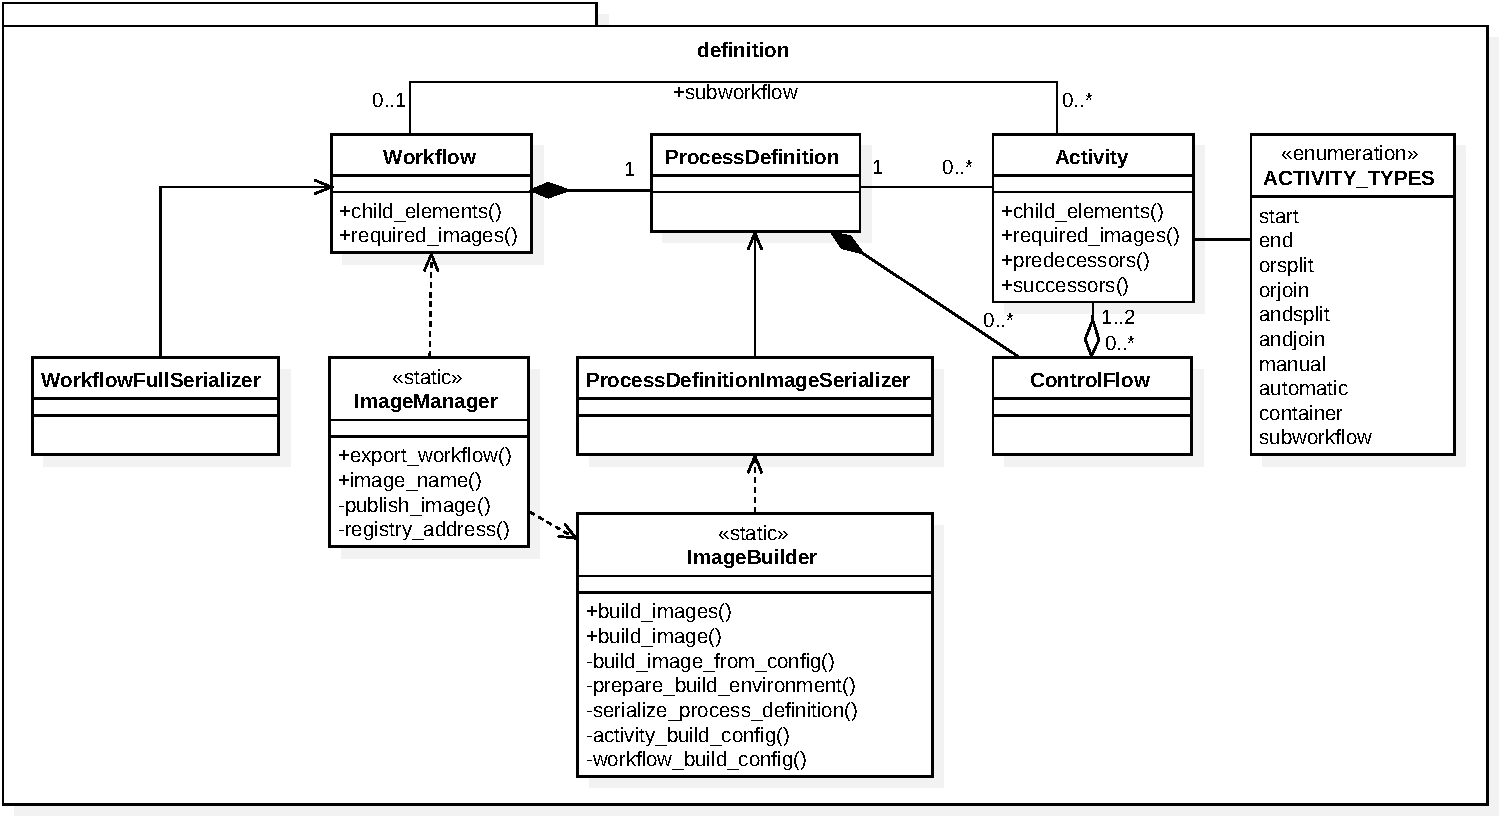
\includegraphics[width=0.95\textwidth]{content/images/class_diagram_definition-crop.pdf}
      \caption*{\scriptsize Controllers omitted for the sake of simplicity. Workflow, ProcessDefinition, Activity and ControlFlow each have a controller with the respective pluralized name plus a `Controller' suffix.}
      \caption{UML Class Diagram for the Definition Service}
      \label{fig:label}
    \end{figure}
    % subsection workflow_definition_service (end)

  \subsection{Organization Management Service} % (fold)
    \label{sub:organization_management_service}
      - application
        - controllers
        - models
          - role
            - ancestors
          - user
            - with role
      - database
        - postgresql
      - data volume
        - docker volume
    % subsection organization_management_service (end)

  \subsection{Worklist Service} % (fold)
    \label{sub:worklist_service}
      - application
        - controllers
        - models
          - worklist item
      - database
        - postgresql
      - data volume
        - docker volume
    % subsection worklist_service (end)

  \subsection{Workflow Engine Service} % (fold)
    \label{sub:workflow_engine_service}
      - application
    % subsection workflow_engine_service (end)

  \subsection{Developer Gateway} % (fold)
    \label{sub:developer_gateway}
      - application
        - backend: rails
        - frontend: angular app
    % subsection developer_gateway (end)

  \subsection{User Gateway} % (fold)
    \label{sub:user_gateway}
      - application
        - backend: rails
        - frontend: angular app
    % subsection user_gateway (end)

  \subsection{Message Oriented Middleware} % (fold)
    \label{sub:message_oriented_middleware}
      For this prototype, RabbitMQ was chosen as message oriented middleware, because it is well documented and has various ruby clients, \eg \emph{Hutch} and \emph{Bunny}.

      RabbitMQ exists as a pre-configured Docker image on the Docker Hub and can thus be utilized easily. The configuration of RabbitMQ in this image takes place when the respective container is run, which allows its configuration in the \texttt{docker-compose} configuration file.
      For the sake of simplicity, no authentication mechanism was introduced besides the simple default username/password combination.
    % subsection message_oriented_middleware (end)

  \subsection{Infrastructure Management Service} % (fold)
    \label{sub:infrastructure_management_service}
      - application
        - app logic
          - docker helper
          - environment manager
        - controllers
          - servers controller
        - models
          - server

    % subsection infrastructure_management_service (end)

  \subsection{Registry} % (fold)
    \label{sub:registry}
    % subsection registry (end)

  \subsection{Provisioning Service} % (fold)
    \label{sub:provisioning_service}
      - application
    % subsection provisioning_service (end)
% section components (end)


\begin{figure}[htbp]
  \centering
  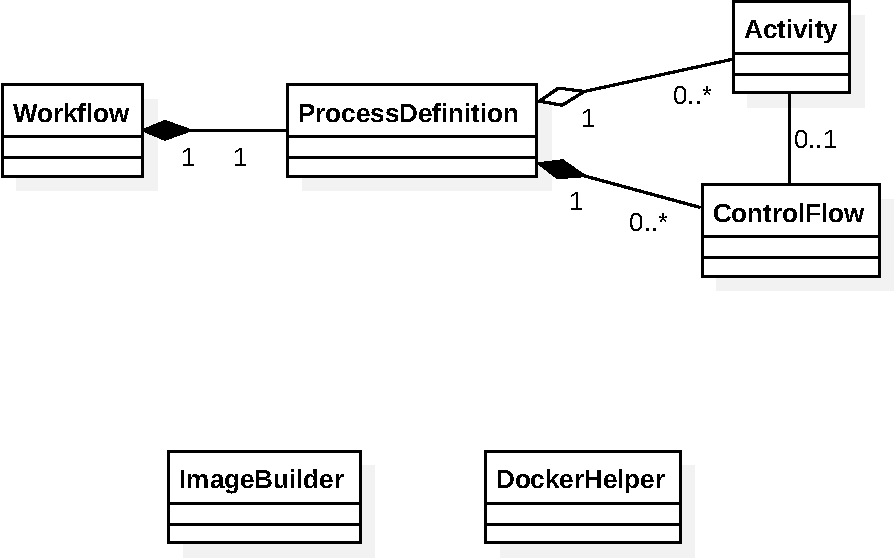
\includegraphics[width=0.95\textwidth]{content/images/class_d_definition-crop.pdf}
  \caption{UML Class Diagram for Workflowe Definition Service}
  \label{fig:uml_class_diagram_definition_service}
\end{figure}

    % chapter implementation (end)

  \chapter{Evaluation and Discussion} % (fold)
    \label{cha:evaluation}
    % -*- root: ../../main.tex -*- %

  - decision tree for wf containerization type -
  - capability table -
  - UML diagrams (classes/deployment) -
  - actual code \& Compose configuration


  In Chapter~\ref{cha:implementation}, the prototypical implementation of a Docker-based \ac{WfMS} is presented. This implementation is based on the considerations that are made in Chapter~\ref{cha:solution_design}. In that chapter, objectives for the prototypical implementation were gathered, together with the requirements that must be met in order for these objectives to be considered fulfilled.

  % Using the prototype, a developer is able to model an organization hierarchy, create workflows and define their processes graphically. These workflows can be exported to Docker containers and are then distributed to all nodes. The developer can start workflows, and -- if a manual activity is present -- a user can enter data. The developer can pause and unpause the workflow.

  In \ref{sub:application_level_communication} is explained how the loose coupling of micro-services via \ac{MOM} and the encapsulation of these services in separate containers can enable alterations to components of the \ac{WfMS} at runtime.

  Regarding the requirements that concern the failure resilience of a service, the prototype is able to let all parts of the system that do not rely on failed services continue to offer their functionality. If, for example, the organization service failed, it would still be possible to model and execute a workflow. Also, the possibility to instruct Docker to restart failed containers can help to keep the system available. In case of a micro-service failure, the unanswered requests to it remain in the queue and can be processed as soon as the service is available again. The prototype's ability to cope with failure can thus mainly be attributed to the combination of Docker with a \ac{MSA}.

  The management of nodes that are available for execution is mostly handled by Docker Swarm. By starting appropriately configured swarm agent containers on them, new nodes may be added to the swarm at any time. The infrastructure service notices the addition of new nodes and starts a provisioning service on them. This service in turn reacts to pushed images and instructs its respective node to pull them.

  The prototype supports the user in using third-party images by providing the means to search for images on the public Docker Hub registry. Further, the invoked command can be specified for utilized third-party images. The graphical modeling environment abstracts from the fact that the container is started by an intermediate activity container.

  % \textbullet ~ User can specify validation  schemas
  % \textbullet ~ \ac{WfMS} performs validity checks

  Some of the objectives were addressed in theory only, but were not implemented in the prototype.
  As described in \ref{sub:execution_scheduling}, nodes can be labeled and these labels can be used to enforce required properties of nodes for certain workflows or activities. ** for single entities?**
  The prototype applies this principle, but in a static way -- not on a dynamic, per-element level.

  Likewise, a solution for the priorization of activities and workflows was presented in \ref{} ** show it**, but it was not implemented in the prototype.

  % An objective that was disregarded in the implementation to keep the *what? thesis short?* is the management of permanently running services which are provided for specific workflows or activities. While it is theoretically described in \ref{}, there is no corresponding functionality in the prototype.

  ** GDVSEPC does not support the exchange of data between workflow instances

  **
  - considering similar functionality /w subworkflow instantiation /validation / etc.    - probably different concept of workflows better as suggested by \cite[119]{Schulze1998Services}
   - recursive structure
   - only one base image

\underline{Note by the author:} With hindsight, the chosen scope would appear too wide for a master thesis with a 70-pages-limitation, leading to shortcuts at places where more in-depth research documentation would have been warranted. Still, the eventual outcome of the paper, i.e. the ultimate decisions on software architecture and -design are founded on solid examination of the available alternatives.

    % chapter evaluation (end)

  \chapter{Conclusion} % (fold)
    \label{cha:conclusion}
    % -*- root: ../../main.tex -*- %

In the thesis at hand, mechanisms and implementation issues that arise from the utilization of Docker and its related tools in the context of \acp{WfMS} were proposed and discussed. Two general application areas for Docker were identified: Docker may influence the architecture and design of \acp{WfMS} as well as provide new ways to distribute and execute workflows.

After introducing the concepts of \ac{WfMS}, Docker and prevalent architecture styles, possibilities for the utilization of Docker for the enactment of workflows were explored. One of them which features the encapsulation of all workflow elements in separate images and a shared data volume, was chosen to be implemented. The attention was then centered on how Docker can be used to create a flexible, failure resilient \ac{WfMS}.

The outcome of these considerations was manifested in the design and implementation of a prototype in which the feasibility of a selection of these mechanisms was demonstrated. In the course of both design and implementation of the prototype, artifacts were created that can be used by succeeding researchers or \ac{WfMS} developers.

results:
  - three promising combinations for execution
  - capability table
  - WfMC model translated to docker-enabled microservices
  - statically compiled activity/workflow would be faster

outlook:
  - pause + move containers: http://blog.circleci.com/checkpoint-and-restore-docker-container-with-criu/
  - evaluate supported patterns?  http://www.workflowpatterns.com/documentation/documents/BPM-06-22.pdf
  - implement resource management


    % chapter conclusion (end)

  \bibliographystyle{plain}
  \bibliography{Remote}
\end{document}
